%CHAPTER
\chapter{Uživatelská dokumentace}
Pro nasazení modulu na webový server je potřeba provést tyto kroky:
\begin{enumerate}
	\item V~kořenovém adresáři serveru nebo v~aktuálním pracovním adresáři je potřeba vytvořit složky \textbf{php} a \textbf{php/offline-review}.
	\item Přesunout celý modul do adresáře \textbf{php/offline-review}.
	\item V~souboru \textit{orlib.php} přepsat konstantu \uv{DATA\_ROOT} na aktuální pracovní adresář či kořenový adresář (přednastavený pracovní adresář je definován v~konfiguračním souboru webového portálu konference TSD).
\end{enumerate}


Postup pro uživatele při využití tohoto modulu:
\begin{enumerate}
	\item Přihlášení do webového portálu konference TSD.
	\item Přesunout se do záložky \uv{My Reviews}.
	\item Vybrat si ze seznamu jeden vědecký příspěvek a kliknout na příslušné tlačítko pro otevření hodnotícího formuláře (\uv{Review} tlačítko).
	\item Pod textem \uv{Offline review form} (v~pravé horní části webového prohlížeče) lze vidět 2 tlačítka:
	\begin{itemize}
		\item Levé tlačítko (obrázek bez zelené šipky) má za úkol vygenerovat příslušný hodnotící soubor k~aktuálně hodnocenému vědeckému příspěvku, viz \ref{fig:download}.
		\item Pravé tlačítko (obrázek se zelenou šipkou) má za úkol zpracovat příslušný hodnotící soubor a nahrát do databáze extrahované hodnotící parametry, viz \ref{fig:upload}.
	\end{itemize}
\end{enumerate}

\begin{figure}[h!]
\centering
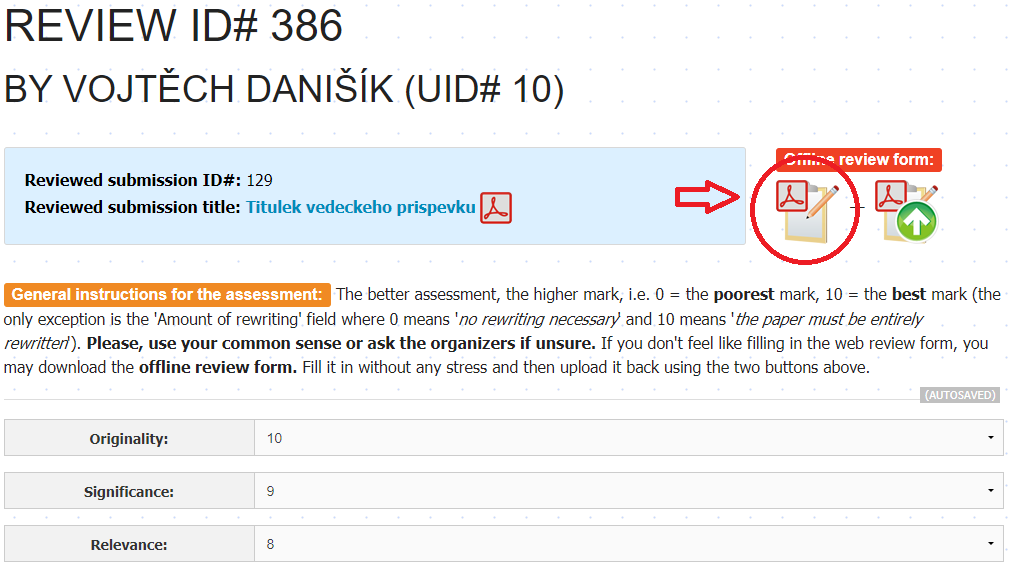
\includegraphics[width=12cm]{img/download}
\caption{Ukázka stažení hodnotícího PDF souboru}
\label{fig:download}
\end{figure}

\begin{figure}[h!]
\centering
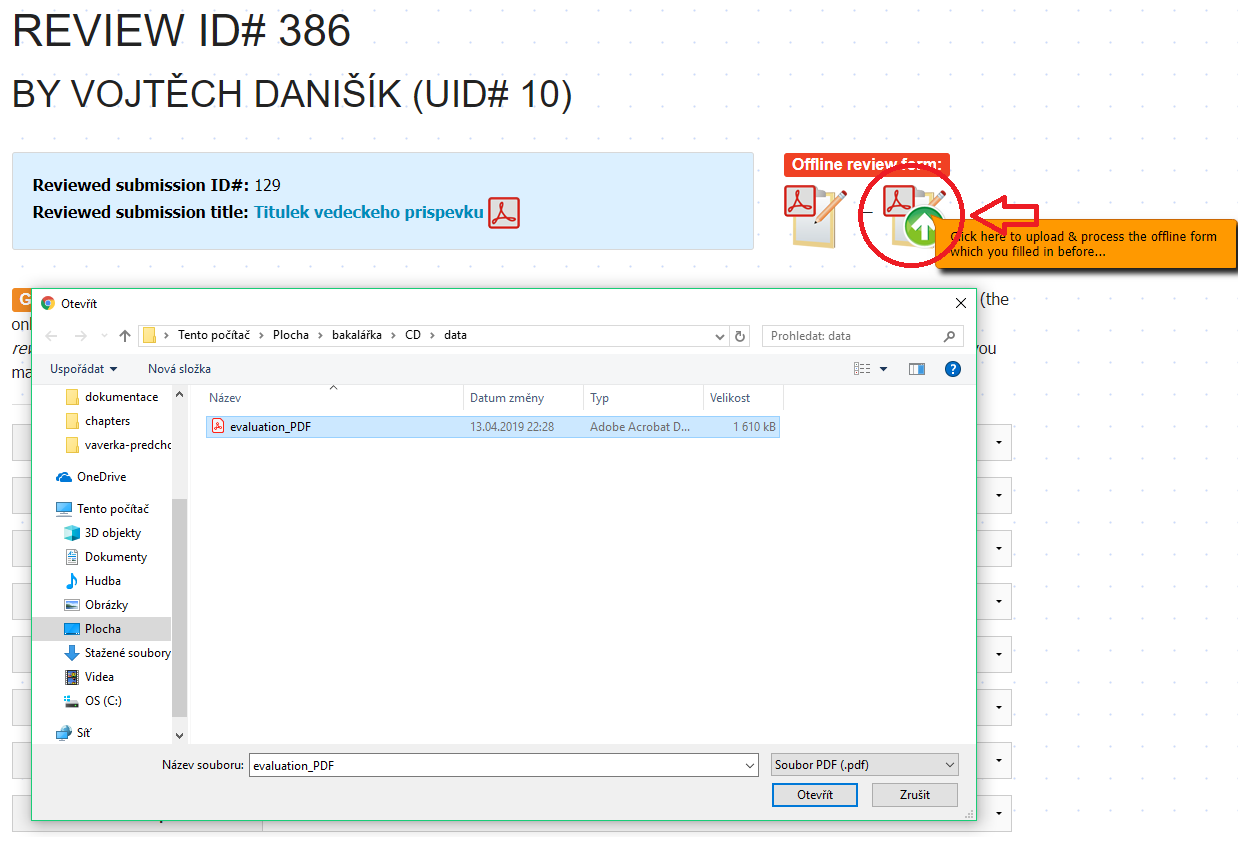
\includegraphics[width=12cm]{img/upload}
\caption{Ukázka nahrání hodnotícího PDF souboru}
\label{fig:upload}
\end{figure}


 